\chapter{評価}
\label{evaluation}
本研究では、本システムを利用することでポーズが改善できるかの検証、また、既存の練習方法である鏡を用いた練習との比較を行うため、
練習前と練習後のポーズの比較と、各ポーズにおけるシステム利用群と鏡利用群の比較を行った。
\section{評価内容}
今回はシステムでのフィードバックでは両肘、両肩の角度についてフィードバックを行なっていたため、評価の際も同様に両肘、両肩の角度について評価を行った。


肩の角度 \(\theta_{\text{肩}}\) は、上腕の単位ベクトル \(\vec{u}\) と両肩を結ぶ線の単位ベクトル \(\vec{w}\) を用いて計算することができる。この角度は、以下の式で定義される:

\[
\theta_{\text{肩}} = \arccos\left( \frac{\vec{u} \cdot \vec{w}}{\|\vec{u}\| \|\vec{w}\|} \right) \times \frac{180}{\pi}
\]


同様に、肘の角度 \(\theta_{\text{肘}}\) は、前腕の単位ベクトル \(\vec{v}\) と上腕の単位ベクトル \(\vec{u}\) を使用して次のように計算される:

\[
\theta_{\text{肘}} = \arccos\left( \frac{\vec{v} \cdot \vec{u}}{\|\vec{v}\| \|\vec{u}\|} \right) \times \frac{180}{\pi}
\]

\section{測定方法}
練習前、練習後、練習から24時間後に写真を撮影し、それをMediapipe Poseを用い、ポーズを解析し角度を測定した。
今回はMediapipe PoseでもBlazePose GHUM Heavyモデルを用いた。BlazePose GHUM Heavyは表 \ref{tab:pose-estimation-quality} に示す通り同じBlazePose GHUのモデルや、AlphaPose ResNet50、Apple Visionと比較しても様々なアクティビティにおいて精度が高いことが報告されている。
この評価で用いられているPCK@0.2とは、人体の各部位の予測点と実際の点の距離が、人体の幅の20\%以内にあるかどうかを判定する指標である。\cite{PCK} また、利用者の属する地域別の精度は \ref{fig:Model-Accuracy-by-Race} に示す。今回の被験者の所属する日本は、Eastern Asiaに属するが、Eastern Asiaでの精度は今回利用するHeavyモデルではPDJという手法で92.6\%となっている。PDJはPCK@0.2と同義である。

\begin{table}[ht]
  \centering
  \begin{tabular}{|l|c|c|c|}
  \hline
  \textbf{Method} & \textbf{Yoga} & \textbf{Dance} & \textbf{HIIT} \\
                  & PCK@0.2       & PCK@0.2        & PCK@0.2       \\ 
  \hline
  BlazePose GHUM Heavy                                                      & \textbf{96.4} & \textbf{97.2} & \textbf{97.5} \\
  BlazePose GHUM Full                                                       & \textbf{95.5} & \textbf{96.3} & \textbf{95.7} \\
  BlazePose GHUM Lite                                                       & \textbf{90.2} & \textbf{92.5} & \textbf{93.5} \\
  \href{https://github.com/MVIG-SJTU/AlphaPose}{AlphaPose ResNet50}         & \textbf{96.0} & \textbf{95.5} & \textbf{96.0} \\
  \href{https://developer.apple.com/documentation/vision/detecting_human_body_poses_in_images}{Apple Vision} & \textbf{82.7} & \textbf{91.4} & \textbf{88.6} \\
  \hline
  \end{tabular}
  \caption{様々なアクティビティにおける様々なモデルのPCK@0.2の比較 \cite{pose-estimation-quality}}
  \label{tab:pose-estimation-quality}
\end{table}
  
\begin{figure}[H]
  \begin{center}
  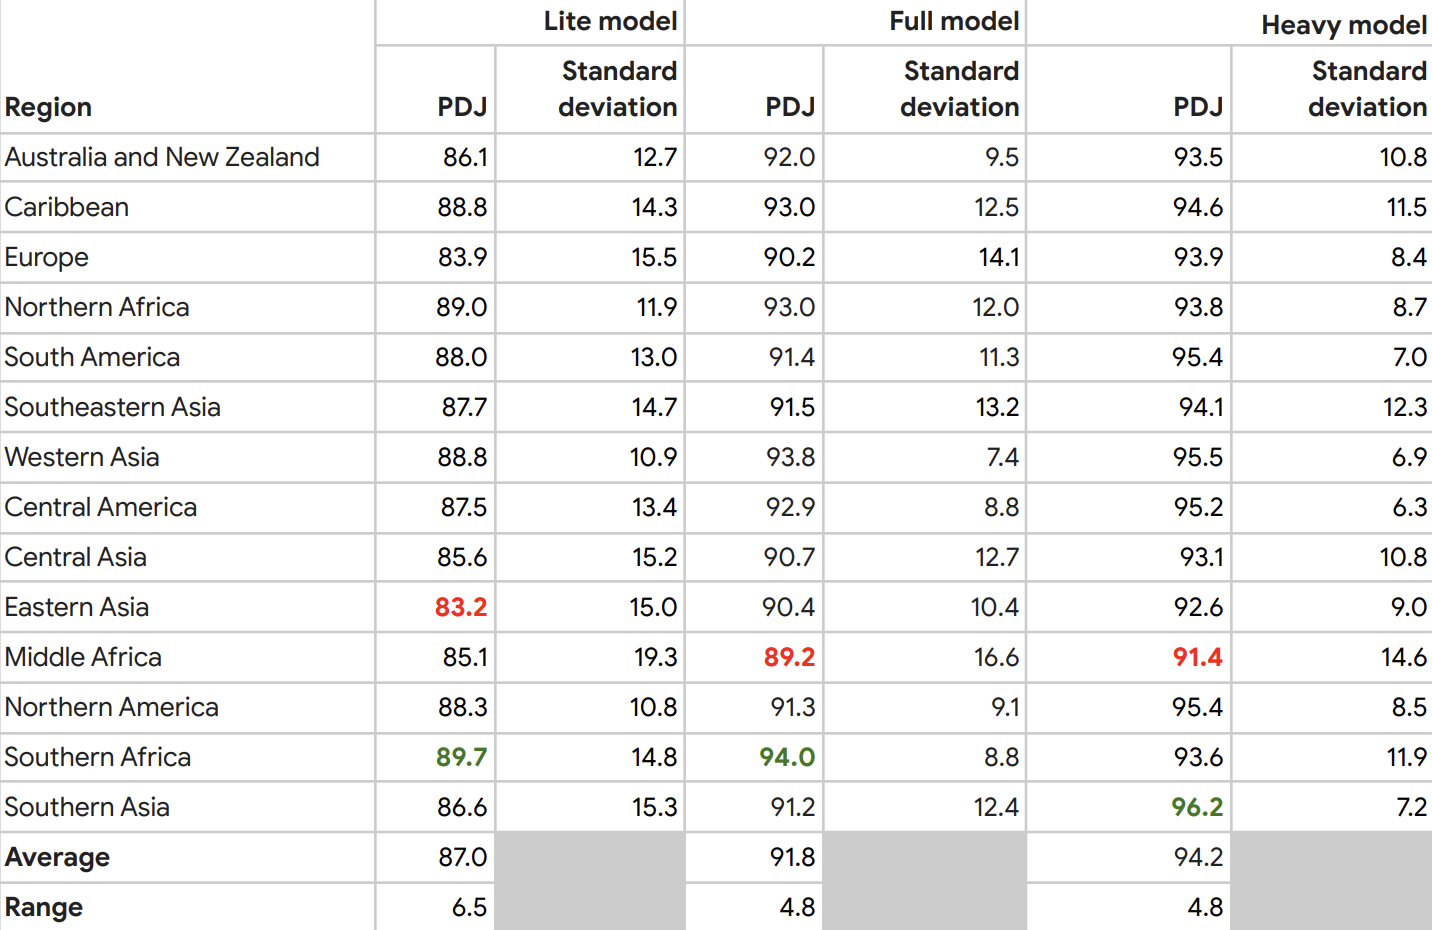
\includegraphics[width=9cm]{figures/Model_Accuracy_by_Race.png}
  \caption{地域別の精度 \cite{Model-Accuracy-by-Race}}
  \label{fig:Model-Accuracy-by-Race}
  \end{center}
\end{figure}

\section{結果}
本研究では練習で改善されたかどうかを評価したいため、練習前、練習後、練習から24時間後のポーズの角度と理想とするポーズの角度の差\(\bar{\theta}_{\text{angle\_dif}}\)を利用して評価する。
それぞれの関節を右肘(RE)、左肘(LE)、右肩(RS)、左肩(LS)とし、以下のように定義した。

\[
  \bar{\theta}_{\text{angle\_dif}} = \frac{1}{4} \sum_{i \in \{\text{RE, LE, RS, LS}\}} |\theta_{i, \text{Actual}} - \theta_{i, \text{Ideal}}|
\]

\subsection{練習前後、24時間後の比較}
ここではシステムを利用して練習した群と鏡を利用して練習した群それぞれの練習前後、24時間後のポーズの理想の角度との差を比較する。
\subsubsection{システム利用群の比較}
TODOここに比較を書く。グラフは木曜日以降
グラフは全被験者の理想との差の平均の3系列棒グラフ、pre→after→24hの順の折れ線グラフを書きたい
\subsubsection{鏡利用群の比較}
TODOここに比較を書く。グラフは木曜日以降
グラフはシステム利用群の比較と同じ

\section{鏡利用群とシステム利用群の比較}
TODOここでは同じポーズにおいてシステム利用群と鏡利用群の比較を行う。グラフは木曜日以降


